\section{Flux de données}
\subsection{Entrée et sortie standard}
\begin{frame}{Entrée et sortie standard}
  \begin{columns}
    \begin{column}{6cm}
      \begin{block}{Rappel : Les programmes informatiques}
        \begin{itemize}
        \item Un programme prend des données en entrée. Ces données
          peuvent être lues dans un fichier ou fournies par un flux du
          système.
        \item Le programme manipule ces données.
        \item Le programme fournit un résultat en sortie (des
          données). Ces données peuvent être écrites dans un fichier ou
          exportées comme un flux vers le système.
        \end{itemize}
      \end{block}
    \end{column}
    \begin{column}{6cm}
      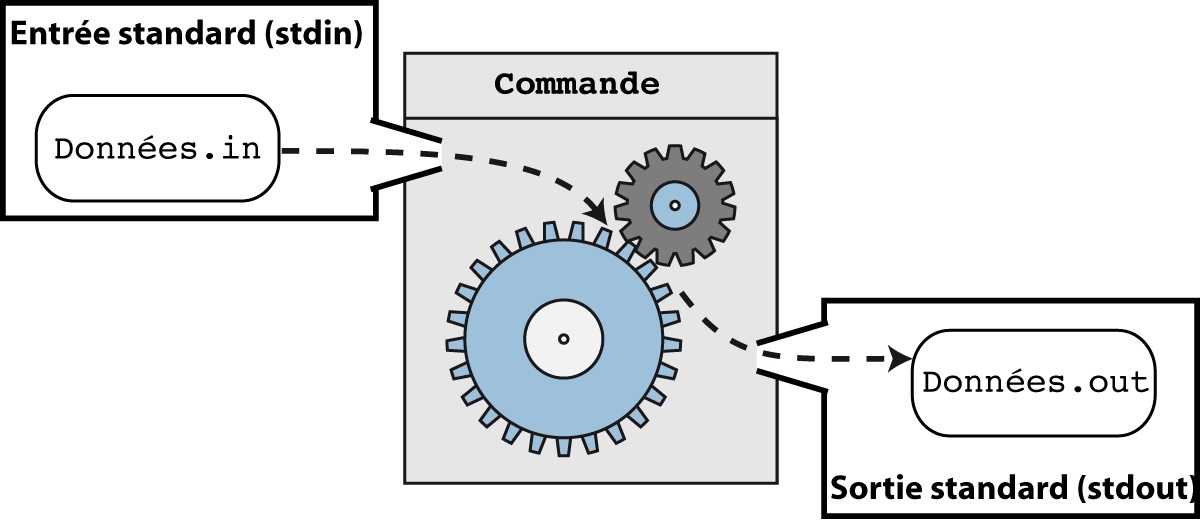
\includegraphics[width=6cm]{img/s05/stdin_stdout_commande_1.jpg}
    \end{column}
  \end{columns}
  \begin{block}{Les flux de données}
    Pour fonctionner, un programme a donc besoin de lire des données
    (flux d'entrée: input) et d'écrire les résultats de ses évaluations
    (flux de sortie: output). On distingue 3 types de flux de données:
    \begin{itemize}
    \item \textbf{STDIN}: entrée standard (là où sont lues les données),
    \item \textbf{STDOUT}: sortie standard (là où sont écrits les
      résultats),
    \item \textbf{STDERR}: sortie erreur (là où sont écrit les messages
      d'erreur).
    \end{itemize}
  \end{block}
\end{frame}
\begin{frame}{Entrée et sortie standard}
  \begin{block}{Les commandes qui lisent sur l'entrée standard}
    \begin{itemize}
    \item Certaines commandes Linux qui traitent les données d'un
      fichier (dont le chemin est passé en paramètre) peuvent
      alternativement, si aucun chemin fichier n'est spécifié,
      travailler directement avec les données lues sur l'entrée
      standard.
    \item Par exemple: \lin{echo}, \lin{cat}, \lin{head}, \lin{tail},
      \lin{grep}.
    \item {\color{red}\textbf{Par défaut, l'entrée standard est le
          clavier}}.
    \end{itemize}
  \end{block}
  \begin{center}
    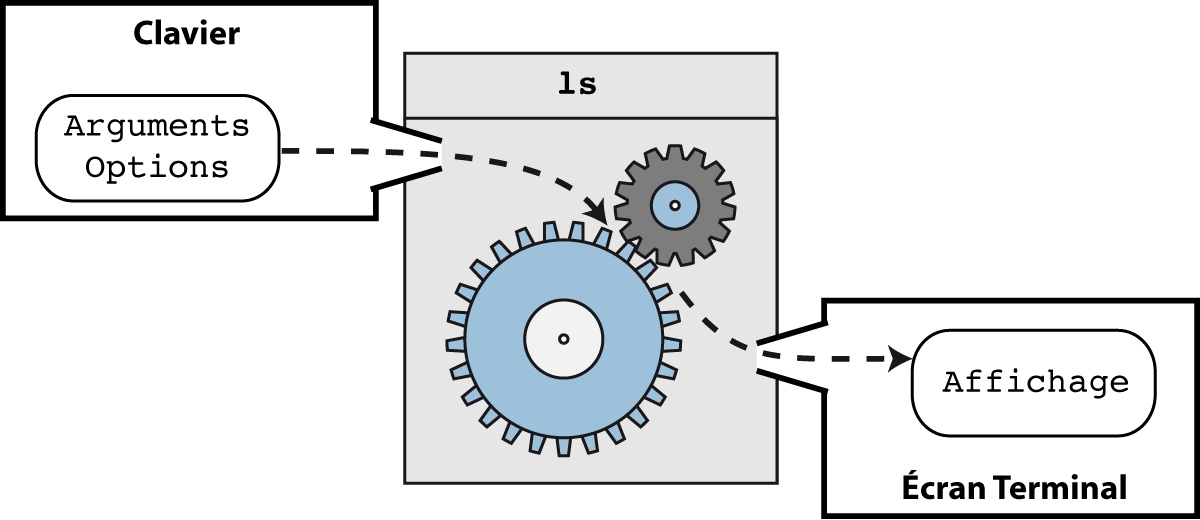
\includegraphics[width=6cm]{img/s05/stdin_stdout_commande_2.jpg}
  \end{center}
  \begin{block}{Les commandes qui écrivent sur la sortie standard}
    \begin{itemize}
    \item Les affichages produits par les commandes Linux sont le
      résultat de leur évaluation. Ce résultat est écrit sur la sortie
      standard.
    \item {\color{red}\textbf{Par défaut, la sortie standard est
          l'écran}}.
    \end{itemize}
  \end{block}
\end{frame}

%%%%%%%%%%%%%%% 

\manpage{cat}

\manpage{head}

\manpage{tail}

\manpage{grep}

\begin{exercice}
  \begin{exercicelet}{Manipulation du contenu d'un fichier texte}
    \begin{questions}
    \item La commande suivante montre le contenu d'un fichier texte:
      \begin{center}
        \small{ \mprompt{ \prompt[\~\//]{cat /proc/cpuinfo}{} } }
      \end{center}
    \item Quelle sont les informations contenues dans ce fichier?
    \item À l'aide des commandes \lin{cat} ou \lin{less} identifiez dans
      le fichier /proc/cpuinfo le nombre de fois ou le mot 'cpu'
      apparait
    \item La commande \lin{grep 'cpu' /proc/cpuinfo} permet d'afficher
      les lignes du fichier \lin{/proc/cpuinfo} où le mot 'cpu'
      apparait. Vérifiez qu'il y en le bon nombre?
    \item L'option -v permet d'inverser son comportement. Au lieu
      d'afficher les lignes qui présentent le motif, \lin{grep} affiche
      alors les lignes qui ne présentent pas le motif. Affichez les
      lignes du fichier \lin{/proc/cpuinfo} ne présentant pas le mot
      'cpu'.
    \item Proposez une commande permettant d'afficher les premières 5
      lignes
    \item Proposez une commande permettant d'afficher les dernières 5
      lignes
    \end{questions}
  \end{exercicelet}
\end{exercice}

%%%%%%%%%%%%%% 
\subsection{Redirections}
\begin{frame}{Redirection des Entrée/Sorties}
  \begin{block}{Commandes de Redirection}
    Il est possible de modifier le comportement par défaut des commandes
    et de donner une entrée et/ou une sortie standard différente des
    entrées/sorties standards.
    \begin{itemize}
    \item \mpromptS{\lin{command > fichier.out}}
      \begin{itemize}
      \item \textbf{{\color{solarizedRed}Redirige la sortie standard}} de la
        commande \lin{command} vers le fichier \lin{fichier.out}.
      \item Si le fichier \lin{fichier.out} n'existe pas, il est créé
        avec comme contenu les affichages produits par la commande
        \lin{command}.
      \item \textbf{{\color{solarizedBlue}Si le fichier \lin{fichier.out}
            existe, son contenu est écrasé}} et remplacé par les
        affichages produits par la commande \lin{command}.
      \end{itemize}
    \item \mpromptS{\lin{command >> fichier.out}}
      \begin{itemize}
      \item \textbf{{\color{solarizedRed}Redirige la sortie standard}} de la
        commande \lin{command} vers le fichier \lin{fichier.out}.
      \item Si le fichier \lin{fichier.out} n'existe pas, il est créé
        avec comme contenu les affichages produits par la commande
        \lin{command}.
      \item Si le fichier \lin{fichier.out} existe, les affichages
        produits par la commande \lin{command} sont
        \textbf{{\color{solarizedBlue}ajoutés à la fin du contenu du
            fichier}}.
      \end{itemize}
    \item \mpromptS{\lin{command 2> fichier.err}}
      \begin{itemize}
      \item \textbf{{\color{solarizedRed}Redirige la sortie erreur}} de la
        commande \lin{command} vers le fichier \lin{fichier.err}
        \textbf{{\color{solarizedBlue}avec écrasement du contenu}} si le
        fichier de sortie existe déjà.
      \end{itemize}
    \item \mpromptS{\lin{command 2>> fichier.err}}
      \begin{itemize}
      \item \textbf{{\color{solarizedRed}Redirige la sortie erreur}} de la
        commande \lin{command} vers le fichier \lin{fichier.err}
        \textbf{{\color{solarizedBlue}avec préservation du contenu}} si le
        fichier de sortie existe déjà.
      \end{itemize}
    \end{itemize}
  \end{block}
\end{frame}
%%%%%%%%%%%%%% 
\begin{frame}{Exemple de redirection}
  \begin{columns}
    \begin{column}{5.5cm}
      \begin{block}{Comportement par défaut de la commande \lin{ls}}
      \end{block}
      \begin{center}
        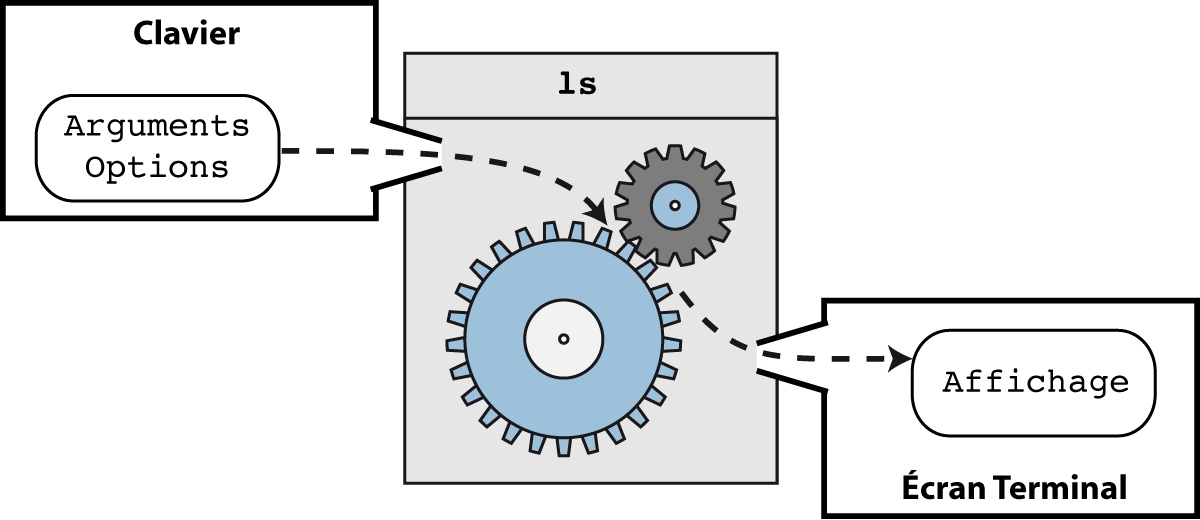
\includegraphics[width=5cm]{img/s05/stdin_stdout_commande_2.jpg}
      \end{center}
      \scriptsize{ \mpromptS{%
          \promptS{ls}{aldenaran.jpg alphacentauri.gif etacentauri.jpg}
          \promptS{ls}{aldenaran.jpg alphacentauri.gif etacentauri.jpg}
          \promptS{\cursor}{} } } La sortie standard de la première
      commande \lin{ls} est l'écran. La liste du contenu du répertoire
      courant est affichée à l'écran.\\\vspace{20pt}
    \end{column}
    \begin{column}{5.5cm}
      \begin{alertblock}{Redirection de la sortie de la commande
          \lin{ls}}
      \end{alertblock}
      \begin{center}
        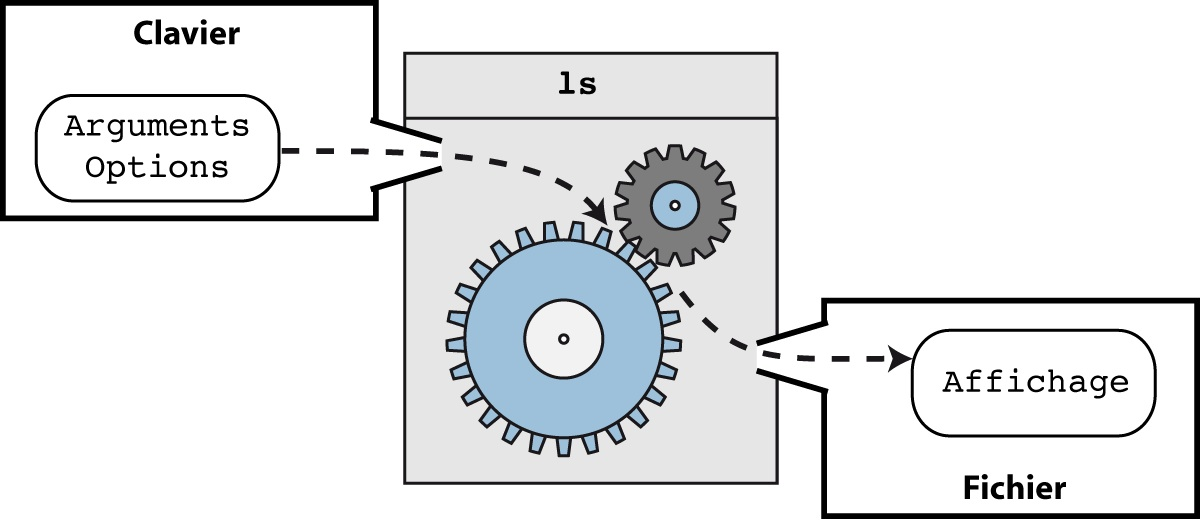
\includegraphics[width=5cm]{img/s05/stdin_stdout_commande_3.jpg}
      \end{center}
      \scriptsize{ \mpromptS{%
          \promptS{ls > {\color{solarizedBlue}1.out}}{}
          \promptS{ls}{{\color{solarizedBlue}1.out} aldenaran.jpg
            alphacentauri.gif etacentauri.jpg} \promptS{\cursor}{} } }
      La sortie standard de la première commande \lin{ls} est redirigée vers le fichier \lin{{\color{solarizedBlue}1.out}}. La liste du contenu du répertoire courant est écrite dans le fichier \lin{{\color{solarizedBlue}1.out}}.\\
      La deuxième commande \lin{ls}, montre qu'un fichier portant le nom
      \lin{{\color{solarizedBlue}1.out}} a été créé.\\\vspace{2pt}
    \end{column}
  \end{columns}
\end{frame}

%%%%%%%%%%%%%%%%%%%%%%%% 

\manpage{echo}

%%%%%%%%%%%%%%%%%%%%%%%% 

\begin{exercice}
  \begin{exercicelet}{Redirections}
    \begin{questions}
    \item Que font les commandes suivantes?
      % \begin{center}
      \small{ \mprompt{ \prompt{echo ``Bonjour"}{} \prompt{echo
            ``Bonjour" > bonjour.out}{} \prompt{echo ``Salut" >
            bonjour.out}{} \prompt{echo ``Bonjour" >> bonjour.out}{} }}
      % \end{center}
    \item Entrainez-vous avec les commandes suivantes. Profitez-en pour
      comprendre les affichages produits par les commandes \lin{ps} et
      \lin{file}:
      \begin{center}
        \mprompt{ \prompt{ps > essai\_ps.out}{} \prompt{file
            /usr/include/stdio.h > file.out}{} }
      \end{center}
    \item Proposez une commande pour copier le contenu de /proc/cpuinfo
      dans un fichier cpuinfo.out sans utiliser la commande \lin{cp}
    \end{questions}
  \end{exercicelet}
\end{exercice}

%%%%%%%%%%%%%% 
\subsection{Tubes}
\begin{frame}{Tubes}
  \begin{block}{Principes de fonctionnement des Tubes (Pipe en anglais)}
    \begin{itemize}
    \item A la différence des redirections simples qui permettent de
      rediriger la sortie standard d'une commande vers un fichier,
    \item {\color{solarizedRed}Un tube permet de rediriger la sortie standard
        d'une commande vers l'entrée standard d'une autre commande}.
    \end{itemize}
  \end{block}
  \begin{center}
    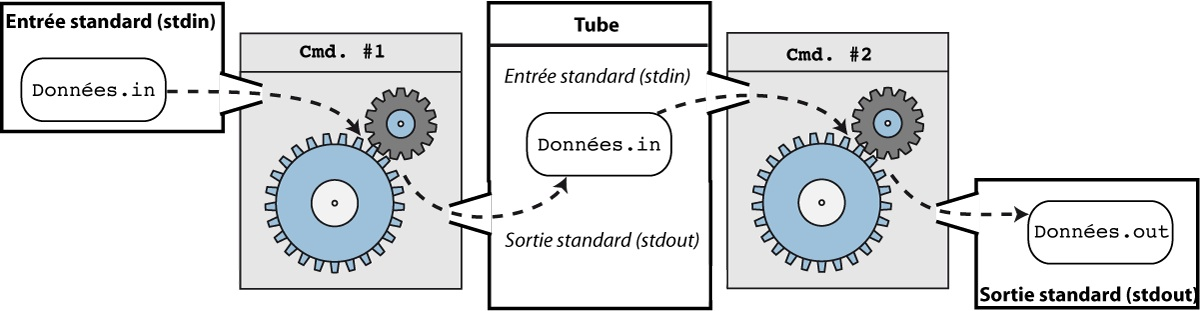
\includegraphics[height=2cm]{img/s05/stdin_stdout_tube_1.jpg}
  \end{center}
  \begin{alertblock}{Syntaxe}
    \begin{itemize}
    \item Le tube est symbolisé par le caractère \lin{|}.
    \item \mpromptS{ \lin{cmd1 | cmd2}}
      \begin{itemize}
      \item La sortie standard de la première commande (\lin{cmd1}) est
        redirigée vers l'entrée standard de la deuxième commande
        (\lin{cmd2}).
      \item L'entrée standard de la commande \lin{cmd1} et la sortie
        standard de la commande \lin{cmd2} ne sont pas modifiées.
      \end{itemize}
    \end{itemize}
  \end{alertblock}
\end{frame}


%%%%%%%%%%%%%% 
\begin{frame}{Exemple de Tubes avec les commande \lin{ls} et \lin{more}}
  \begin{block}{Rappel des commandes:}
    \begin{itemize}
    \item \lin{ls} affiche à l'écran (stdout) la liste des fichiers
      contenus dans un répertoire.
    \item \lin{more} affiche page par page le contenu des données passée
      sur son entrée standard.
    \end{itemize}
  \end{block}
  \begin{alertblock}{Exemple \#1}
    \begin{itemize}
    \item Si de très nombreux fichiers sont contenus dans un répertoire,
      la commande \lin{ls} peut produire un affichage qui ne tient pas
      dans l'écran, rendant impossible le parcours de la liste des
      fichiers (seuls les derniers sont visibles).
    \end{itemize}
    \begin{columns}
      \begin{column}{6cm}
        \small{ \mpromptS{%
            \promptS{ls}{} }\\\vspace{5pt} Défilement de tous les
          fichiers\\\vspace{5pt} \mpromptS{%
            \lin{%aldebaran.jpg alphacentauri.gif\\
              betelgeuse.jpg\hspace{2em}etacentauri.jpg\\soleil.jpg\hspace{4em}syrius.gif\\vega.png}\\
            \promptS{\cursor}{} } }
      \end{column}
      \begin{column}{6cm}
        \dirtree{%
          .1 \DTd{Images}\DTcomment{{\color{solarizedRed}Répertoire courant}}.
          .2 aldebaran.jpg\DTcomment{Hors de la fenetre}.  .2
          alphacentauri.gif\DTcomment{Hors de la fenetre}.  .2
          {\color{solarizedGreen}betelgeuse.jpg}\DTcomment{{\color{solarizedGreen}Dans
              la fenetre}}.  .2 {\color{solarizedGreen}
            etacentauri.jpg}\DTcomment{{\color{solarizedGreen}Dans la
              fenetre}}.  .2 {\color{solarizedGreen}
            soleil.jpg}\DTcomment{{\color{solarizedGreen}Dans la fenetre}}.
          .2 {\color{solarizedGreen}
            syrius.gif}\DTcomment{{\color{solarizedGreen}Dans la fenetre}}.
          .2 {\color{solarizedGreen}
            vega.png}\DTcomment{{\color{solarizedGreen}Dans la fenetre}}.
        }
      \end{column}
    \end{columns}
  \end{alertblock}
\end{frame}


%%%%%%%%%%%%%% 
\begin{frame}{Exemple de Tubes avec les commande \lin{ls} et \lin{more}}
  \begin{alertblock}{Exemple \#1 (suite):}
    \begin{itemize}
    \item La redirection de la sortie standard de la commande \lin{ls}
      vers l'entrée standard de la commande \lin{more} permet de passer
      en revue l'affichage de la commande \lin{ls} page par page.
    \end{itemize}
    \begin{center}
      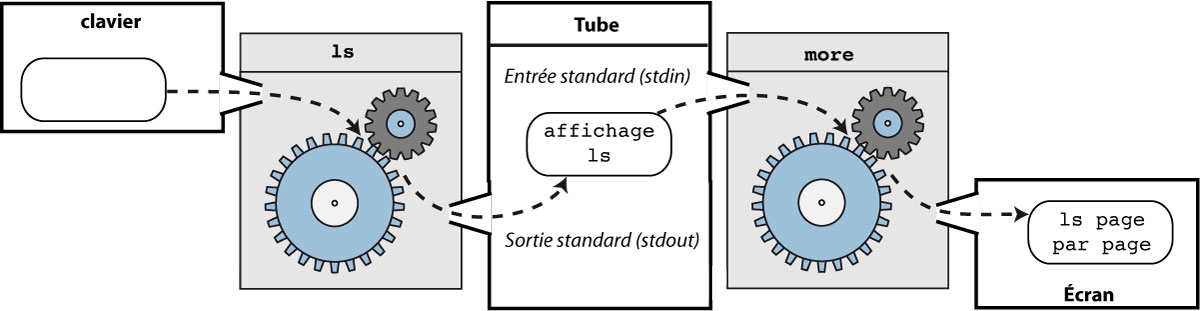
\includegraphics[height=2cm]{img/s05/stdin_stdout_tube_ls_more.jpg}
    \end{center}
    \begin{columns}
      \begin{column}{6cm}
        \small{ \mpromptS{%
            \promptS{ls | more}{aldebaran.jpg\hspace{2.5em}alphacentauri.gif\\
              betelgeuse.jpg\hspace{2em}etacentauri.jpg\\soleil.jpg\hspace{4em}syrius.gif}
          }\\
          Affichage d'une première page puis \\
          Presser la touche \Enter pour la page suivante\\
          \mpromptS{%
            \lin{soleil.jpg\hspace{4em}syrius.gif\\vega.png}\\
            \promptS{\cursor}{} } }
      \end{column}
      \begin{column}{6cm}
        \dirtree{%
          .1 \DTd{Images}\DTcomment{{\color{solarizedRed}Répertoire courant}}.
          .2 aldebaran.jpg\DTcomment{Page 1}.  .2
          alphacentauri.gif\DTcomment{Page 1}.  .2
          betelgeuse.jpg\DTcomment{Page 1}.  .2
          etacentauri.jpg\DTcomment{Page 1}.  .2
          soleil.jpg\DTcomment{Page 1\&2}.  .2 syrius.gif\DTcomment{Page
            1\&2}.  .2 vega.png\DTcomment{Page 2}.  }
      \end{column}
    \end{columns}
  \end{alertblock}
\end{frame}

%%%%%%%%%%%%%% 
\begin{frame}{Exemple de Tubes avec les commande \lin{ls} et \lin{grep}}
  \begin{block}{Rappel des commandes:}
    \begin{itemize}
    \item \lin{ls} affiche à l'écran (stdout) la liste des fichiers
      contenus dans un répertoire.
    \item \lin{grep} affiche les lignes d'un texte qui comportent un
      certain motif.
    \end{itemize}
  \end{block}
  \begin{alertblock}{Exemple \#2:}
    \begin{itemize}
    \item Si de très nombreux fichiers sont contenus dans un répertoire,
      la commande \lin{ls} peut produire un affichage qui ne tient pas
      dans l'écran, rendant compliqué l'identification de certain type
      de fichier (fichiers au format \lin{gif} par exemple).
    \end{itemize}
    \begin{columns}
      \begin{column}{6cm}
        \small{ \mpromptS{%
            \promptS{ls}{aldebaran.jpg\\alphacentauri.gif\\betelgeuse.jpg\\etacentauri.jpg\\soleil.jpg\\syrius.gif\\vega.png}
            \promptS{\cursor}{} } }
      \end{column}
      \begin{column}{6cm}
        \dirtree{%
          .1 \DTd{Images}\DTcomment{{\color{solarizedRed}Répertoire courant}}.
          .2 aldebaran.jpg\DTcomment{Affiché}.  .2
          alphacentauri.gif\DTcomment{Affiché}.  .2
          betelgeuse.jpg\DTcomment{Affiché}.  .2
          etacentauri.jpg\DTcomment{Affiché}.  .2
          soleil.jpg\DTcomment{Affiché}.  .2
          syrius.gif\DTcomment{Affiché}.  .2
          vega.png\DTcomment{Affiché}.  }
      \end{column}
    \end{columns}
  \end{alertblock}
\end{frame}

%%%%%%%%%%%%%% 
\begin{frame}{Exemple de Tubes avec les commande \lin{ls} et \lin{more}}
  \begin{alertblock}{Exemple \#2 (suite):}
    \begin{itemize}
    \item La redirection de la sortie standard de la commande \lin{ls}
      vers l'entrée standard de la commande \lin{grep} permet
      d'effectuer un filtrage des fichiers présents dans le répertoire
      sur la base d'un motif présent dans leur nom (par exemple
      l'extension \lin{.gif}).
    \end{itemize}
    \begin{center}
      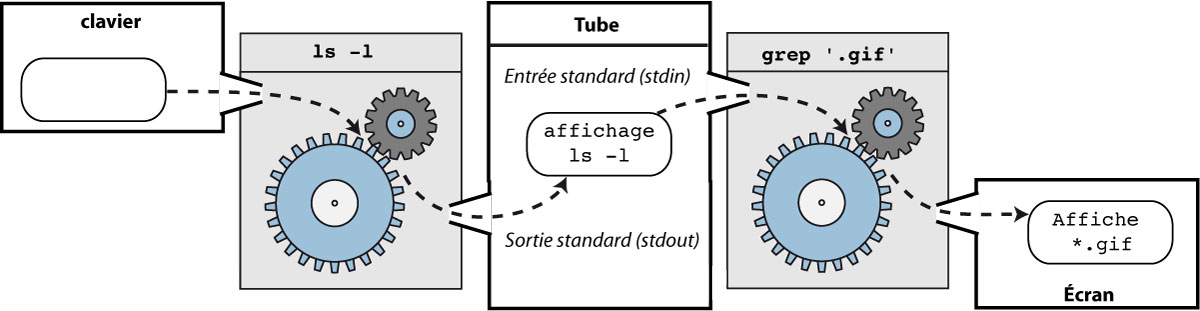
\includegraphics[height=2cm]{img/s05/stdin_stdout_tube_ls_grep.jpg}
    \end{center}
    \begin{columns}
      \begin{column}{6cm}
        \small{ \mpromptS{%
            \promptS{ls | grep '.gif'}{alphacentauri.gif\\syrius.gif}
            \promptS{\cursor}{} } }
      \end{column}
      \begin{column}{6cm}
        \dirtree{%
          .1 \DTd{Images}\DTcomment{{\color{solarizedRed}Répertoire courant}}.
          .2 aldebaran.jpg\DTcomment{Retenu par le filtre}.  .2
          alphacentauri.gif\DTcomment{Affiché}.  .2
          betelgeuse.jpg\DTcomment{Retenu par le filtre}.  .2
          etacentauri.jpg\DTcomment{Retenu par le filtre}.  .2
          soleil.jpg\DTcomment{Retenu par le filtre}.  .2
          syrius.gif\DTcomment{Affiché}.  .2 vega.png\DTcomment{Retenu
            par le filtre}.  }
      \end{column}
    \end{columns}
  \end{alertblock}
\end{frame}

%%%%%%%%%%%%%% 

\manpage{wc}

%%%%%%%%%%%% 

\begin{exercice}
  \begin{exercicelet}{Tubes}
    \begin{questions}
    \item Étudiez et comparez les commandes suivantes. Pour vous aider
      vous pouvez évaluer les commandes pas à pas en vous arrêtant avant
      chaque tube.
      % \begin{center}
      \small{ \mprompt{ \prompt{cat /proc/cpuinfo | wc -l}{}
          \prompt{head /proc/cpuinfo | wc -l}{} \prompt{cat
            /proc/cpuinfo | grep 'cpu' | wc -l}{} \prompt{head
            /proc/cpuinfo | grep 'cpu' | wc -l}{} }}
      % \end{center}
    \item Proposez une commande pour afficher le nombre de fichiers dans
      votre répertoire home
    \item Proposez une commande pour afficher le nombre des processus
    \item Proposez une commande pour afficher les premières 5 lignes des
      dernières 10 lignes du fichier /proc/cpuinfo
    \end{questions}
  \end{exercicelet}
\end{exercice}

